\documentclass[11pt]{article}
\pagestyle{plain}
\usepackage{xcolor}
\usepackage{lipsum}
\usepackage{setspace}
\renewcommand{\baselinestretch}{1.25} 
\usepackage{calc}
\usepackage{graphicx} 
\reversemarginpar
   \usepackage{graphicx}
\usepackage[paper=letterpaper, 
            marginparwidth=0.1in, 
            marginparsep=.1in, 
            margin=0.4in,
            left=0.4in,%
            right=0.4in,%
            includemp]{geometry}

\setlength{\parindent}{0in}

\usepackage[shortlabels]{enumitem}
% ============================================================
%:Markup macros for proof-reading
\usepackage{ifthen}
\usepackage[normalem]{ulem} % for \sout
\usepackage{xcolor}
\newcommand{\ra}{$\rightarrow$}
\newboolean{showedits}
\setboolean{showedits}{true} % toggle to show or hide edits
%\setboolean{showedits}{false} % toggle to show or hide edits
\ifthenelse{\boolean{showedits}}
{
	\newcommand{\meh}[1]{\textcolor{red}{\uwave{#1}}} % please rephrase
	\newcommand{\ins}[1]{\textcolor{blue}{\uline{#1}}} % please insert
	\newcommand{\del}[1]{\textcolor{red}{\sout{#1}}} % please delete
	\newcommand{\chg}[2]{\textcolor{red}{\sout{#1}}{\ra}\textcolor{blue}{\uline{#2}}} % please change
	\newcommand{\nbe}[3]{
		{\colorbox{#3}{\bfseries\sffamily\scriptsize\textcolor{white}{#1}}}
		{\textcolor{#3}{\sf\small$\blacktriangleright$\textit{#2}$\blacktriangleleft$}}}
}{
	\newcommand{\meh}[1]{#1} % please rephrase
	\newcommand{\ins}[1]{#1} % please insert
	\newcommand{\del}[1]{} % please delete
	\newcommand{\chg}[2]{#2}
	\newcommand{\nbe}[3]{}
}
%
\newcommand\rA[1]{\nbe{Reviewer A}{#1}{cyan}}
\newcommand\rB[1]{\nbe{Reviewer B}{#1}{olive}}
\newcommand\rC[1]{\nbe{Reviewer C}{#1}{magenta}}
\newcommand\ANS[1]{\nbe{Response}{#1}{teal}}
% ============================================================
%:Put edit comments in a really ugly standout display
%\usepackage{ifthen}
\usepackage{amssymb}
\newboolean{showcomments}
\setboolean{showcomments}{true}
%\setboolean{showcomments}{false}
\newcommand{\id}[1]{$-$Id: scgPaper.tex 32478 2010-04-29 09:11:32Z oscar $-$}
\newcommand{\yellowbox}[1]{\fcolorbox{gray}{yellow}{\bfseries\sffamily\scriptsize#1}}
\newcommand{\triangles}[1]{{\sf\small$\blacktriangleright$\textit{#1}$\blacktriangleleft$}}
\ifthenelse{\boolean{showcomments}}
%{\newcommand{\nb}[2]{{\yellowbox{#1}\triangles{#2}}}
{\newcommand{\nbc}[3]{
 {\colorbox{#3}{\bfseries\sffamily\scriptsize\textcolor{white}{#1}}}
 {\textcolor{#3}{\sf\small$\blacktriangleright$\textit{#2}$\blacktriangleleft$}}}
 \newcommand{\version}{\emph{\scriptsize\id}}}
{\newcommand{\nbc}[3]{}
 \newcommand{\version}{}}
\newcommand{\nb}[2]{\nbc{#1}{#2}{orange}}
\newcommand{\here}{\yellowbox{$\Rightarrow$ CONTINUE HERE $\Leftarrow$}}
\newcommand\rev[2]{\nb{TODO (rev #1)}{#2}} % reviewer comments
\newcommand\fix[1]{\nb{FIX}{#1}}
\newcommand\todo[1]{\nb{TO DO}{#1}}
\newcommand\on[1]{\nbc{ON}{#1}{red}} % add more author macros here
%\newcommand\XXX[1]{\nbc{XXX}{#1}{blue}}
%\newcommand\XXX[1]{\nbc{XXX}{#1}{brown}}
%\newcommand\XXX[1]{\nbc{XXX}{#1}{cyan}}
%\newcommand\XXX[1]{\nbc{XXX}{#1}{darkgray}}
%\newcommand\XXX[1]{\nbc{XXX}{#1}{gray}}
%\newcommand\XXX[1]{\nbc{XXX}{#1}{magenta}}
%\newcommand\XXX[1]{\nbc{XXX}{#1}{olive}}
%\newcommand\XXX[1]{\nbc{XXX}{#1}{orange}}
%\newcommand\XXX[1]{\nbc{XXX}{#1}{purple}}
%\newcommand\XXX[1]{\nbc{XXX}{#1}{red}}
%\newcommand\XXX[1]{\nbc{XXX}{#1}{teal}}
%\newcommand\XXX[1]{\nbc{XXX}{#1}{violet}}
% ============================================================


\makeatletter
\newlength{\bibhang}
\setlength{\bibhang}{1em}
\newlength{\bibsep}
 {\@listi \global\bibsep\itemsep \global\advance\bibsep by\parsep}
\newlist{bibsection}{itemize}{3}
\setlist[bibsection]{label=,leftmargin=\bibhang,%
        itemindent=-\bibhang,
        itemsep=\bibsep,parsep=\z@,partopsep=0pt,
        topsep=0pt}
\newlist{bibenum}{enumerate}{3}
\setlist[bibenum]{label=[\arabic*],resume,leftmargin={\bibhang+\widthof{[99]}},%
        itemindent=-\bibhang,
        itemsep=\bibsep,parsep=\z@,partopsep=0pt,
        topsep=0pt}
\let\oldendbibenum\endbibenum
\def\endbibenum{\oldendbibenum\vspace{-.6\baselineskip}}
\let\oldendbibsection\endbibsection
\def\endbibsection{\oldendbibsection\vspace{-.6\baselineskip}}
\makeatother


\usepackage{fancyhdr,lastpage}
\pagestyle{fancy}
%\pagestyle{empty}      % Uncomment this to get rid of page numbers
\fancyhf{}\renewcommand{\headrulewidth}{0pt}
\fancyfootoffset{\marginparsep+\marginparwidth}
\newlength{\footpageshift}
\setlength{\footpageshift}
          {0.2\textwidth+0.2\marginparsep+0.2\marginparwidth-2in}
%\lfoot{\hspace{\footpageshift}%
%       \parbox{2in}{\, \hfill %
%                    \arabic{page} of \protect\pageref*{LastPage} % +LP
%%                    \arabic{page}                               % -LP
%                    \hfill \,}}

% Finally, give us PDF bookmarks
\usepackage{color,hyperref}
\definecolor{darkblue}{rgb}{0.0,0.0,0.3}
\hypersetup{colorlinks,breaklinks,
            linkcolor=darkblue,urlcolor=darkblue,
            anchorcolor=darkblue,citecolor=darkblue}


\newcommand{\makeheading}[2][]%
        {\hspace*{-\marginparsep minus \marginparwidth}%
         \begin{minipage}[t]{\textwidth+\marginparwidth+\marginparsep}%
             {\large \bfseries #2 \hfill #1}\\[-0.15\baselineskip]%
                 \rule{\columnwidth}{1pt}%
         \end{minipage}}

\renewcommand{\section}[1]{\pagebreak[3]%
    \vspace{1.3\baselineskip}%
    \phantomsection\addcontentsline{toc}{section}{#1}%
    \noindent\llap{\scshape\smash{\parbox[t]{\marginparwidth}{\hyphenpenalty=10000\raggedright #1}}}%
    \vspace{-\baselineskip}\par}

\newcommand*\fixendlist[1]{%
    \expandafter\let\csname preFixEndListend#1\expandafter\endcsname\csname end#1\endcsname
    \expandafter\def\csname end#1\endcsname{\csname preFixEndListend#1\endcsname\vspace{-0.6\baselineskip}}}

\let\originalItem\item
\newcommand*\fixouterlist[1]{%
    \expandafter\let\csname preFixOuterList#1\expandafter\endcsname\csname #1\endcsname
    \expandafter\def\csname #1\endcsname{\csname preFixOuterList#1\endcsname\let\oldItem\item\def\item{\pagebreak[2]\oldItem}}
    \expandafter\let\csname preFixOuterListend#1\expandafter\endcsname\csname end#1\endcsname
    \expandafter\def\csname end#1\endcsname{\let\item\oldItem\csname preFixOuterListend#1\endcsname}}
\newcommand*\fixinnerlist[1]{%
    \expandafter\let\csname preFixInnerList#1\expandafter\endcsname\csname #1\endcsname
    \expandafter\def\csname #1\endcsname{\let\oldItem\item\let\item\originalItem\csname preFixInnerList#1\endcsname}
    \expandafter\let\csname preFixInnerListend#1\expandafter\endcsname\csname end#1\endcsname
    \expandafter\def\csname end#1\endcsname{\csname preFixInnerListend#1\endcsname\let\item\oldItem}}
 
\newlist{outerlist}{itemize}{3}
    \setlist[outerlist]{label=\enskip\textbullet,leftmargin=*}
    \fixendlist{outerlist}
    \fixouterlist{outerlist}

\newlist{lonelist}{itemize}{3}
    \setlist[lonelist]{label=\enskip\textbullet,leftmargin=*,partopsep=0pt,topsep=0pt}
    \fixendlist{lonelist}
    \fixouterlist{lonelist}

\newlist{innerlist}{itemize}{3}
    \setlist[innerlist]{label=\enskip\textbullet,leftmargin=*,parsep=0pt,itemsep=0pt,topsep=0pt,partopsep=0pt}
    \fixinnerlist{innerlist}

\newlist{loneinnerlist}{itemize}{3}
    \setlist[loneinnerlist]{label=\enskip\textbullet,leftmargin=*,parsep=0pt,itemsep=0pt,topsep=0pt,partopsep=0pt}
    \fixendlist{loneinnerlist}
    \fixinnerlist{loneinnerlist}

\newcommand{\blankline}{\quad\pagebreak[3]}
\newcommand{\halfblankline}{\quad\vspace{-0.5\baselineskip}\pagebreak[3]}

\newcommand\doilink[1]{\href{http://dx.doi.org/#1}{#1}}
\newcommand\doi[1]{doi:\doilink{#1}}

\providecommand*\url[1]{\href{#1}{#1}}
\renewcommand*\url[1]{\href{#1}{\texttt{#1}}}
\providecommand*\email[1]{\href{mailto:#1}{#1}}
\providecommand\BibTeX{{B\kern-.05em{\sc i\kern-.025em b}\kern-.08em
    \TeX}}
\providecommand\Matlab{\textsc{Matlab}}
\hyphenation{bio-mim-ic-ry bio-in-spi-ra-tion re-us-a-ble pro-vid-er}

\pagenumbering{roman}

\begin{document}
\pagenumbering{roman}
%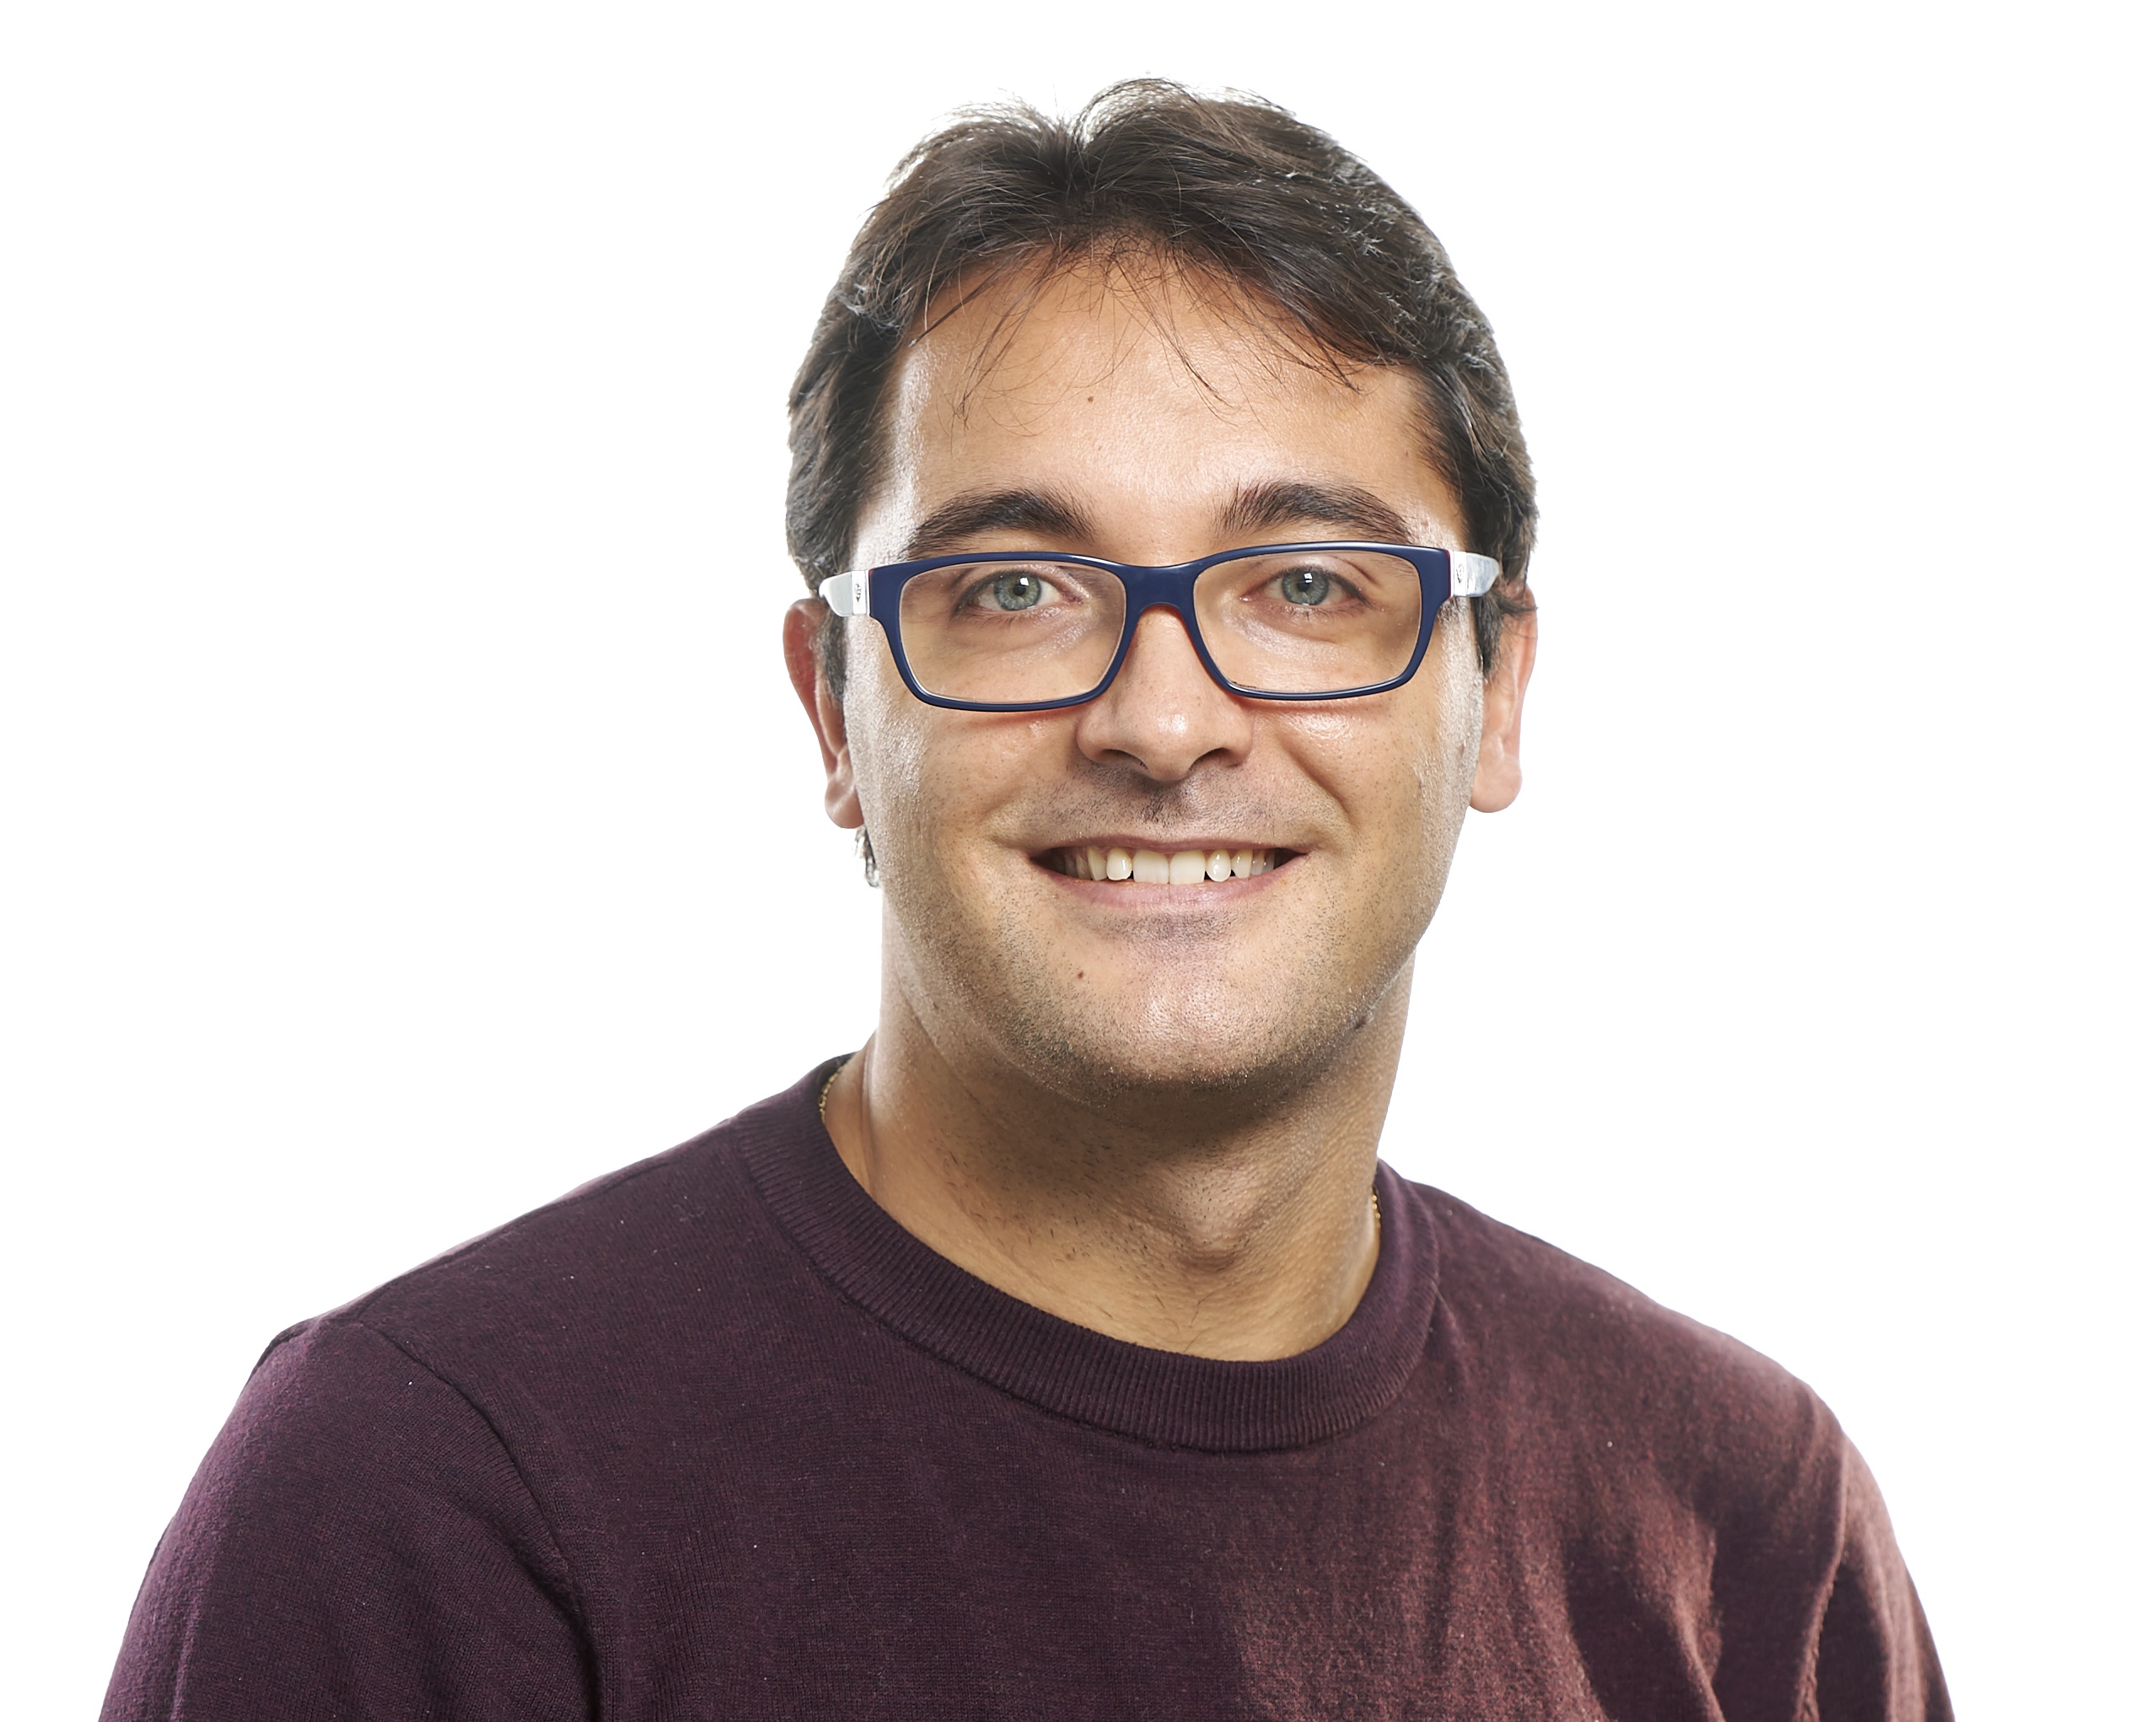
\includegraphics[width=3.3cm, height=3.5cm]{images/s_panichella.jpg}\\
\vspace{-2mm}
\textsc{\fontsize{13}{12}\selectfont Sebastiano Panichella - Curriculum vitae \& major scientific achievements}\\
\vspace{-2mm}

%\newlength{\rcollength}\setlength{\rcollength}{1in}%
%\newlength{\spacewidth}\setlength{\spacewidth}{20pt}
%\newcommand\spacechar{$|$}

\noindent\begin{minipage}{0.2\textwidth}% adapt widths of minipages to your needs
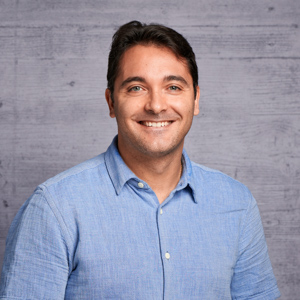
\includegraphics[width=3.11cm, height=3cm]{images/PANC.jpg}
\end{minipage}%
\hfill%
\begin{minipage}{0.9\textwidth}\raggedright
\textsc{Contact Information}\\
{\small
%\textit{Address:} Department of Computer Engineering\\ \href{http://www.ing.unisannio.it/}{University of Sannio}\\
%RCOST- Palazzo ex Poste, Via Traiano\\
%82100 Benevento (Italy).\\\\
%\textit{Mobile:} +39 3881969673\\
%\textit{Tel.: +39 0824 305539} \\
%\textit{E-mail:} \email{spanichella@gmail.com}\\
%\textit{Home Page:} \href{http://www.ing.unisannio.it/spanichella}{www.ing.unisannio.it/spanichella}
\textit{Address:} \href{}{University of Bern (UniBe)}\\ 
Schützenmattstrasse 14, 3012 Bern, Switzerland.\\ 
%\textit{Tel.: +39 0824 305539} \\
%\textit{Tel.: +41 (0) 58 934 41 56} \\
\textit{E-mail:} \email{sebastiano.panichella@unibe.ch} (or alternatively \email{spanichella@gmail.com})\\
\textit{Home Page:} \href{https://spanichella.github.io/}{https://spanichella.github.io/}\\
\textit{Google Scholar Ref:}\\ \url{https://scholar.google.it/citations?user=HiNuBFgAAAAJ\&hl=en\&oi=ao}\\
\textit{CV:} \href{https://spanichella.github.io/img/CV.pdf}{https://spanichella.github.io/img/CV.pdf}\\
%\textit{Detailed CV:} \href{https://spanichella.github.io/img/CV.pdf}{https://spanichella.github.io/img/CV.pdf}}\\
\end{minipage}


\vspace{2.5mm}
\textsc{Education}
\vspace{1.5mm}

Sebastiano Panichella was born in Italy.
He received the PhD in Computer Science from the University of Sannio 
 defending the thesis entitled  \href{http://dx.doi.org/10.1109/ICSM.2015.7332519}{\textit{``Supporting Newcomers in Open Source Software Development Projects"}} (\textbf{July 18th 2014}). \textbf{Supervisors}: Prof. Massimiliano  Di Penta and Prof. Gerardo Canfora.

\vspace{2.5mm}
\textsc{Employment history \& Institutional responsibilities}
\vspace{1.5mm}
%During the PhD his work was supervised by 
%Prof. Gerardo Canfora and 
%Prof. Massimiliano Di Penta and Prof. Gerardo Canfora.

%\textbf{Major scientific achievements}
%\vspace{1mm}

Currently, he is a Senior Computer Science Researcher at the University of Bern (from \textit{\textbf{09-2024}}). Previously he was a Senior Computer Science Researcher and Lecturer in Software Engineering at ZHAW (from 08-2018 to 08-2024), a postdoc at the University of Zurich (\textbf{2014-11-01 - 2018-08-19}) in the lab of Prof Gall and part-time (External) Lecturer at the University of Zurich (between \textit{\textbf{2018-2022}}). \\
His main \textbf{research goal} is to conduct industrial research, involving both industrial and academic collaborations, to sustain the Internet of Things (IoT) vision, where future "smart cities" will be characterized by millions of smart systems and AI-enabled systems (e.g., cyber-physical systems such as drones, and other autonomous and intelligent systems) connected over the internet, composed by AI-components, and/or controlled by complex embedded software implemented for the cloud.
Sebastiano Panichella is also deeply interested in \textbf{interdisciplinary research}, where computer science intersects with life sciences. His work bridges software engineering, AI/ML, and domain-specific expertise, creating impactful collaborations beyond traditional disciplinary boundaries.
\\
%\medskip\\ 
His  \textbf{research interests}\footnote{ Research interests detailed here \url{https://spanichella.github.io/research\_interests.html}} are in the domain of Software Engineering (SE), cloud computing (CC), and Data Science (DS): DevOps (e.g., Continuous Delivery, Continuous Integration), Machine learning applied to SE, Software maintenance and evolution (with particular focus on Cloud, mobile, AI-based, and Cyber-physical applications). 
He authored or co-authored \textbf{more than one hundred} (considering also demonstration, dataset, poster) papers that appeared in International Conferences and Journals (26 of them published during the postdoctoral experience at the University of Zurich).
 

\vspace{2.5mm}


\textsc{\fontsize{14}{12}\selectfont Major scientific achievements}


\noindent \textbf{Achievement 1 - Funding, Leadership of Projects, and Related Impact}. 
In the last decade, He has demonstrated his ability to receive (competitive) funding (for a \textbf{total over 3,500,000 CHF}) and lead projects as a PI
and co-PI, on topics related to AI and Data Science (e.g., Mobile Computing, life sciences, robotics, etc.), Mining Software
Repositories, DevOps and MLOps, Human-computer Interactions, Software Maintenance, and
Software Development, Evolution, and Testing for Cyber-physical and AI Systems:

\vspace{-3.5mm}
\begin{itemize}

  \item PI (at UniBe) of the Horizon EU  "Marie Sklodowska-Curie Actions-funded Doctoral Networks" for the project "InnoGuard: Hybrid and Generative Intelligence for Trustworthy Autonomous Cyber-Physical Systems".
\textbf{Total project around 5MIL EUR. Budget for UniBe is of 607,132.8 EUR (595,779.42 CHF)}. Web page: \href{https://www.innoguard.eu/index.html}{https://www.innoguard.eu/index.html}
\vspace{-2.5mm}
  \item PI of the H2020 EU project COSMOS: ``DevOps for Complex Cyber-physical Systems". \textbf{Total H2020 project 5MIL EUR, Sebastiano Panichella got direct funding for 770,000 EUR}. \\Web page: \href{https://www.cosmos-devops.org/}{https://www.cosmos-devops.org/}
\vspace{-2.5mm}
\item PI for   the project ``SwarmOps: Human-sensing based MLOps for Collaborative Cyber-physical systems" (2024-2028).  \textbf{Total project 667,280 CHF}.  Web page: \href{https://spanichella.github.io/projects.html}{https://spanichella.github.io/projects.html}
\vspace{-2.5mm}
\item PI for the Innosuisse project  "BioAI4LCMS: Automated LC-MS through AIbased and Generative Intelligence Technology Application" \textbf{Total project 1.2 MIL CHF (working hours allocated to it), Sebastiano Panichella got direct funding for around 350,000 CHF}
\vspace{-2.5mm}
  \item PI of the Innosuisse project ``ARIES: Exploiting User Journeys and Testing Automation for Supporting Efficient Energy Service Platforms". \textbf{Total project funding: \textbf{500,000 CHF} (538,660 EUR)}. Web page: \href{https://spanichella.github.io/projects/aries-devops/index.html}{https://spanichella.github.io/projects/aries-devops/index.html}
\vspace{-2.5mm}
  \item Co-PI for
   the SURF-MobileAppsData SNF project. \textbf{Total SNSF (CHF) 471,018}. 
   %\\Web page: \href{http://www.ifi.uzh.ch/en/seal/people/panichella/SNF-Projects.html}{http://www.ifi.uzh.ch/en/seal/people/panichella/SNF-Projects.html}
\vspace{-2.5mm}
   \item PI for the Doctoral funding at the SoE ZHAW. \textbf{Total project funding:\textbf{114,000 CHF} (122,814 EUR)}.
\vspace{-2.5mm}
  \item PI for a Hasler Foundation Project "AERIALIST: Bridging the Reality Gap in Testing Unmanned Aerial Vehicles".  
\textbf{Total project 50,000 CHF (53,866 EUR)}. \\Web page: \href{https://skhatiri.github.io/Aerialist-Project/}{https://skhatiri.github.io/Aerialist-Project/} 
\vspace{-2.5mm}
  \item Co-PI for a Hasler Foundation Project (co-applicant with Atefeh Rohani) "Safe-2-Fly: Advancing Unmanned Aerial Vehicles Reliability and Societal Trust Through Integrated Testing and Formal Verification" (Project Number 2025-02-27-311).
\textbf{Total project 50,000 CHF (53,866 EUR)} 
\vspace{-2.5mm}
  \item Sebastiano Panichella got funding (as main research responsible) by two different internal funding calls of the University of Bern. 
The first project is called "Seed funding", aimed at supporting funding acquisition actions of UniBe applicants for Horizon projects.
The second project is for "Interdisciplinary teaching": UniBe is supporting Sebastiano Panichella's teaching initiatives on courses between Robotics, AI, Software Engineering, and the Faculty of Laws (concerning e.g., regulatory aspects and ethics in AI and autonomous cyber-physical systems).
\textbf{Total of the two internal projects 24,000 CHF (working hours allocated to it), Sebastiano Panichella got direct funding for around 17,000 CHF}
\vspace{-2.5mm}
  \item \textbf{Complete list of past and ongoing projects can be found at}:  https://spanichella.github.io/projects.html
\vspace{-3.5mm}
\end{itemize}


In terms of funding, here some impact indicators:
\begin{itemize}
  \item \textbf{F-Index (in EUR)}: (funding / 1000) / number of years after the PhD = \textbf{346}
  \item \textbf{FH-Index (in EUR)}: (funding / 1000) / h-index = \textbf{83}
  \item \textbf{Avg-Citations}: Nr. total citations / Nr. of Publications = \textbf{67 citations per paper}
\end{itemize}

Key factors attracting collaborations and funding are his team's accessible, impactful, and replicable research results. Notable examples include frameworks for developing, testing and monitoring the safety/behavior of UAVs and SDCs, published in top-tier conferences and journals, which are 
%,  and 
widely adopted in industry (e.g., Anybotics) and academia.  Here are some selected international events where such frameworks are adopted as part of new tool competitions: 
%through sensor-based and digital twin analyses. They also highlights the new tool competitions organized at
%international events where he has served as general/workshop chair):  %Here are some selected events:  
%A key aspect that attracts collaborations and funding are his accessible and replicable research results. Tangible examples are the frameworks widely used by academia and industry, developed as follow-up development activities of approaches proposed in top publications in A and A* conferences and top journals. His team has developed frameworks now used as a reference to test and monitor the safety states of Unmanned aerial vehicles (UAVs) and self-driving cars (SDCs), which requires both sensor-based and digital twins analysis of simulated and real autonomous systems. These frameworks are at the core of new and original tool competitions organized in past and recent international events, where he acted as general/workshop chair:
\begin{itemize}
{\fontsize{11}{11.5}\selectfont 
\vspace{-2.5mm}
	%\item https://shonan.nii.ac.jp/seminars/204/ - 
    %\vspace{-2.5mm}
	%\item https://conf.researchr.org/committee/icst-2025/icst-2025-organizing-committee
    %\vspace{-2.5mm}
	\item https://conf.researchr.org/track/icst-2025/icst-2025-tool-competition--self-driving-car-testing
    \vspace{-2.5mm}
	\item https://conf.researchr.org/track/icst-2025/icst-2025-tool-competition--uav-testing
    \vspace{-2.5mm}
	\item https://sbft25.github.io/tools/ ,  https://sbft24.github.io/tools/ , https://sbft23.github.io/tools/ , etc. %https://sbst22.github.io/
    \vspace{-3mm}
	\item https://nlbse2024.github.io/index.html , https://nlbse2023.github.io/tools/ 
    }
\end{itemize}
\vspace{-2.5mm}
The ideas, approaches, and tools developed in his projects\footnote{https://spanichella.github.io/tools.html} are shaping research directions in the DevOps and MLOps fields and have already had an impact. As a tangible example, the European Commission's Innovation Radar Assessment of the project stated that the innovations developed in the COSMOS H2020 project\footnote{https://www.cosmos-devops.
org/} have been analyzed by the European Commission's Innovation Radar\footnote{https://innovation-radar.ec.europa.eu/} and categorized as "Market Maturity" and "Market
Ready"\footnote{https://innovation-radar.ec.europa.eu/methodology/\#maturity-info} as reported in the
selected EU portal\footnote{https://innovation-radar.ec.europa.eu/innovation/57508}. Very few projects
have been marked with such an evaluation. The main significance of such recognition consists of a
concrete invitation to build a startup/company on the innovations developed in the COSMOS project.


\vspace{1mm}
\noindent \textbf{Achievement 2 - Contributions to the Research Field, the Community, and Education}
\vspace{-2.5mm}
\begin{itemize} 
\item \textbf{Impact in the Field and the Community:} 
Over the last decade, his projects, research publications, and collaborations have positioned him as a \textbf{\textit{leading researcher in mining software repositories, automated development, testing, and monitoring of cyber-physical systems, AI-enabled systems, and other intelligent systems}}. 
%His work complements research at other Swiss universities. 
His research results are published at leading conferences (e.g., ICSE, ASE, ESEC/FSE, ICST, ICSME, etc.) and internationally renowned software and
systems engineering journals (e.g., TSE, TOSEM, EMSE, JSS, etc.) where his research areas find applications. 
\textbf{In terms of community services}, He regularly serves as the organizer, PC member, and reviewer for international conferences, workshops, and scientific journals, and He is very well-connected and/organizes international events
(conferences and workshops\footnote{https://adevops4iot.github.io/
-	https://sbst22.github.io/ - https://sbft23.github.io/ - https://sbft24.github.io/ -	https://nlbse2022.github.io/ - https://nlbse2023.github.io/ - https://nlbse2024.github.io/}), involving numerous national and international leading scientists
and research institutions in Switzerland and abroad. \textbf{A complete list of his community services can be found at his home page}\footnote{\url{https://spanichella.github.io/teaching\_and\_advising.html}}). 
Complementary, his \textbf{collaborations involve a dense set of flagship companies} such as automotive (AICAS), aviation (GMV), robotics (e.g.,
Anybotics), e-health (Siemens Healthcare), and other intelligent system domains.  \\
\textbf{A complete list of his past, recent, and ongoing collaborations can be found on his home page}\footnote{\url{https://spanichella.github.io/collaborations.html}}). 
Here is a summary of some of his \textbf{\textit{key contributions to the field}}:  
\begin{itemize}
\vspace{-2.5mm}
\item 
\textbf{Mining Software Repositories \& DevOps for Software Systems and CPSs}: He analyzed diverse software data (e.g., Apache projects, mobile app logs) to support development activities. His recent projects have been on AI-based systems and CPSs (e.g., in automotive, healthcare, and robotics), which need better adaptability to dynamic environments. As PI of EU/National projects, He defined DevOps and MLOps practices for testing and monitoring CPSs in critical sectors. Through studies, workshops, and special issues, He explored DevOps, MLOps, and Digital Twin strategies, especially for continuous delivery and test automation for CPSs. Current projects aim to enhance CPS monitoring, leveraging operational data (e.g., sensors, models) for security and safety.

\item 
\textbf{AI for Software Engineering \& Software Engineering for AI-CPSs}: He impacted the field by applying and adapting AI approaches (e.g., ML, NLP) to predict bugs, automate tests, and enable runtime monitoring for complex systems. In his past SNSF and Innosuisse projects, (1) He combined AI and human input analysis to enhance software maintenance and testing for event-based systems; and (2) focused on the development and AI-driven tools for energy-efficient systems. 

\item 
\textbf{Interdisciplinary Research, IoT Vision \& Research Leadership}: His research bridges software engineering, AI/ML, cloud computing, and life sciences to advance the IoT vision, where smart cities will be powered by millions of AI-enabled and autonomous cyber-physical systems (e.g., drones, robotics, healthcare devices). He has authored around one hundred publications (including best papers and book chapters), supervised around 60 students (BSc, MSc, PhD, postdocs, and assistants), and actively contributes to the SE community as PC member of top-tier conferences (e.g., ICSE, ISSTA, ASE, ICSME). His leadership is evidenced by competitive funding achievements of more than 3.5M~CHF as PI or co-PI across Horizon EU, SNSF, Innosuisse, and Hasler Foundation projects. He is also Editorial Board Member of JSEP and TOSEM. His international recognition includes being ranked among the top 2\% scientists worldwide by Stanford University (2022--2025) and in the top 0.5\% by ScholarGPS (2024--2025). In 2025, he received both the ICSME Most Influential Paper Award and the ICST Most Influential 5-Year Journal Paper Award.
\vspace{-2mm}
\end{itemize}


 \item \textbf{Top Selected publications that influenced (or are influencing) the research field}:
\begin{enumerate}
{ 
%\fontsize{9}{9.5}\selectfont 
\vspace{-1.5mm}
\item 
\underline{S. Panichella}, A. Di Sorbo, E. Guzman, A. Visaggio, G. Canfora, H. Gall: 
How Can I Improve My App? Classifying User Reviews for Software Maintenance and Evolution. 
International Conference on Software Maintenance and Evolution. 2015

\item A. Di Sorbo, F. Zampetti, A. Visaggio, M. Di Penta, \underline{S. Panichella}: 
Automated Identification and Qualitative Characterization of Safety Concerns Reported in UAV Software Platforms. 
Transactions on Software Engineering and Methodology. 2022

\item F. Zampetti, R. Kapur, M. Di Penta, \underline{S. Panichella}: 
An Empirical Characterization of Software Bugs in Open-Source Cyber-Physical Systems. 
Journal of Systems \& Software. 2022

\item C. Birchler, S. Khatiri, B. Bosshard, A. Gambi, \underline{S. Panichella}: 
Machine Learning-based Test Selection for Simulation-based Testing of Self-driving Cars Software. 
Empirical Software Engineering. 2023

\item S. Khatiri, \underline{S. Panichella}, P. Tonella: 
Simulation-based Test Case Generation for Unmanned Aerial Vehicles in the Neighborhood of Real Flights. 
International Conference on Software Testing, Verification and Validation. 2023

\item C. Birchler, T. Kombarabettu Mohammed, P. Rani, T. Nechita, T. Kehrer, \underline{S. Panichella}: 
How does Simulation-based Testing for Self-driving Cars match Human Perception? 
ACM International Conference on the Foundations of Software Engineering. 2024

\item C. Birchler, S. Khatiri, P. Rani, T. Kehrer, \underline{S. Panichella}: 
A Roadmap for Simulation-Based Testing of Autonomous Cyber-Physical Systems: Challenges and Future Direction. 
Special issue "A 2030 Roadmap for Software Engineering" in Transactions on Software Engineering and Methodology. 2025

\item S. Khatiri, F. Mohammadi Amin, \underline{S. Panichella}, P. Tonella: 
When Uncertainty Leads to Unsafety: Empirical Insights into the Role of Uncertainty in Unmanned Aerial Vehicle Safety. 
Empirical Software Engineering Journal (EMSE). 2025

\item S. Khatiri, F. Barrientos, M. Wulf, P. Tonella, \underline{S. Panichella}: 
Bridging Research and Practice in Simulation-based Testing of Industrial Robot Navigation Systems. 
International Conference on Automated Software Engineering. 2025

\item \textbf{Selected Contributions to Books}:
  \begin{itemize}
    \item \underline{S. Panichella} (Editor): \textit{Roadmap for DevOps in Cyber-physical Systems: Challenges and Future Directions}. 2025
    \item \underline{S. Panichella} contributions to the book: \textit{Large Language Models in Cybersecurity and Cyberdefense: Novel Threats and Mitigations Perspectives}. 
    Chapters: ``Vulnerabilities Introduced by LLMs through Code Suggestions'', 
    ``Enhancing Security Awareness and Education for Large Language Models''. 2024
  \end{itemize}
}
\vspace{-2mm}
\end{enumerate}
  \vspace{-2mm}
  \item 
  \textbf{Contributions to Education and Supervision of Junior Researchers}\footnote{More details at \url{https://spanichella.github.io/teaching\_and\_advising.html}}:  
%He began teaching as a student assistant at the University of Salerno and later independently during his PhD at the University of Sannio. He has led courses at UZH , ZHAW, where he expanded his teaching to include Software Development, DevOps, Cloud Computing, and Java Programming. At UniBe, he taught the Software Skills Lab (Java, data structures, and algorithms) and co-lectured on Software Engineering (DevOps and AI-based systems). He also supervises student projects and offers research seminars in DevOps and software engineering.
Over the years, he contributed to courses and \textbf{educational chapters and is co-authoring the first book on DevOps for Cyber-Physical Systems''} (targeted for publication in 2025), involving several international researchers. He also authored the \textbf{book "Roadmap for DevOps in Cyber-physical Systems: Challenges and Future Directions"} and contributed chapters in the volume "Large Language Models in Cybersecurity and Cyberdefense: Novel Threats and Mitigations Perspectives" (e.g., Vulnerabilities Introduced by LLMs through Code Suggestions’’ and ``Enhancing Security Awareness and Education for Large Language Models’’). 

He \textbf{supervised or co-supervised} 19 undergraduate students, 27 MSc students, 17 PhD students (6 of them during the postdoctoral experience at the University of Zurich), 10 research assistants, and 1 postdoc. Many of these collaborations resulted in peer-reviewed publications, including award-winning theses such as \textbf{Pooja Rani’s Best PhD Thesis at UniBe in 2023}. Several of his PhD and MSc students have published in highly ranked conferences and journals (e.g., ICSE, ASE, ICSME, TOSEM, EMSE, JSS), and contributed to international tool competitions (ICST, SBFT). 

His teaching contributions range from traditional \textbf{Software Engineering and Software Testing courses} to newly designed \textbf{interdisciplinary teaching programs at UniBe}, such as “DevOps for Cyber-Physical Systems” and “Autonomous Systems in Practice: Technology, Law, and Society” (planned for Spring 2026). He has also developed online courses, such as the Udemy module “Advanced Software Testing, Maintenance and Evolution” (2025).

Beyond education, his mentorship activities emphasize preparing young researchers for both academic and industrial careers, with former students now working as software engineers, researchers, and faculty members worldwide.

  
  \vspace{-2mm} 

\end{itemize}


\noindent \textbf{Achievement 3 - Awards\footnote{https://spanichella.github.io/awards.html}, Tools\footnote{https://spanichella.github.io/tools.html} \& Industrial and Academic Collaborations\footnote{https://spanichella.github.io/collaborations.html}, and other Achievements} 

Ensuring replicability and impactful research results is central to \href{https://spanichella.github.io/collaborations.html}{fostering academic and industrial collaborations}. His approach leverages diverse strategies tailored to diverse partners and research groups, including co-supervision, internships (e.g., Sajad Khatiri's PhD internship at Anybotics), participation in national (Innosuisse/SNSF) and EU (Horizon) projects, and design of courses. Additionally, he organizes conferences and workshops, such as serving as \textit{\textbf{general chair for the 2025 International Conference on Software Testing, Verification, and Validation}}. 
Over the past decade, he built extensive collaborations with industrial and research organizations across various domains, including Genedata (biology computation), Stadler (rail), LEDCity (energy efficiency), Siemens AG and Healthcare (DevOps for ICT/healthcare), and more. His team ensures accessible and replicable research outputs, such as frameworks adopted in academia and industry, derived from top-tier publications in A/A* conferences and journals. 

\vspace{1mm}
 \textbf{Key Achievements and Recognition}:
\begin{itemize}
\vspace{-2mm} 
 \item \textbf{Awards - Complete list at \href{https://spanichella.github.io/awards.html}{https://spanichella.github.io/awards.html
}}: Dr. Sebastiano Panichella published over one hundred papers in international conferences and journals, many of which have earned best paper awards or nominations. He received 4 tools awards (and nominations) as well as 12 best paper awards and best paper nominations. In 2025, he received the \textbf{Most Influential Paper (MIP) Award at ICSME} and the \textbf{Most Influential 5-Years Journal Paper on Software Testing Award at ICST}. 
% \vspace{-2.5mm}
 % \item The paper [\underline{S. Panichella}, A. Di Sorbo, E. Guzman, C. Visaggio, G. Canfora, H. Gall: How can I improve my app? Classifying user reviews for software maintenance and evolution. ICSME 2015], which originated the idea behind his SNSF project, is one of the \textbf{most cited papers of ICMSE 2015} (as reported in Google Scholar), with more than \textbf{600 citations} in 10 years.  
  \vspace{-2.5mm}
\item 
    \textbf{Top Researcher Rankings}: He ranked among the top 20 most impactful software engineering researchers worldwide (2019, 2021) by the Journal of Systems and Software. The report from Stanford University reports him among the top 2\% scientists in his field (2022, 2023, 2025), and he was recognized in the top 0.5\% by ScholarGPS (2024, 2025). 
\item
    \textbf{Editorial and Reviewing Roles}: Dr. Panichella is Editorial Board Member of the \textit{Journal of Software: Evolution and Process (JSEP)} and \textit{ACM Transactions on Software Engineering and Methodology (TOSEM)}. He was recognized as a \textbf{Distinguished Reviewer for TOSEM}. 
 \vspace{-2.5mm}
 \item 
    \textbf{Funding Achievements}: Over the last decade, he has secured more than \textbf{3.5 million CHF} in competitive funding as PI or co-PI from national and international organizations (e.g., Horizon EU, H2020, SNSF, Innosuisse, Hasler Foundation). His projects span AI/ML, DevOps, MLOps, life sciences, robotics, and cyber-physical systems. 
 \vspace{-2.5mm}
 \item 
    \textbf{Innovation and Societal Impact}: The \textbf{COSMOS H2020 project}, coordinated by Dr. Panichella, was evaluated by the \textit{European Commission's Innovation Radar} (2024) and classified as “\textit{Market Ready}” and “\textit{Market Maturity},” highlighting the high transfer potential of his research outcomes.
 \vspace{-2.5mm}
 \item 
    \textbf{Industrial Collaborations}\footnote{\url{https://spanichella.github.io/collaborations.html}}: He established strong collaborations with leading companies across sectors such as robotics (ANYbotics, PAL Robotics), automotive and aerospace (AICAS, Intelligentia, TKMS ATLAS), healthcare and biopharma (Genedata, Siemens Healthcare, Hygeia Hospitals), and software industry leaders (JetBrains, Red Hat, NXP). These partnerships foster knowledge transfer and practical impact. 
 \vspace{-2.5mm}
 %\item 
 %   \textbf{Teaching and Mentorship}: He designed and lectured new interdisciplinary courses at the University of Bern on “\textit{DevOps for Cyber-Physical Systems}” and “\textit{Autonomous Systems in Practice: Technology, Law, and Society}” (planned for 2026). He supervised (or co-supervised) \textbf{over 50 MSc students, 17 PhD students, postdocs, and research assistants}, many of whom have received recognition (e.g., \textbf{Best PhD Thesis Award}, University of Bern, 2025).
\end{itemize}


 \textbf{Collaborative Research Highlights}:
 
\begin{itemize}
\vspace{-2.5mm}
\item 
\textbf{Collaborations:} 
Dr. Panichella has established collaborations with academic and industrial organizations in Switzerland (UniBe, UZH, USI, ETH, ZHAW, etc.) and abroad, such as the USA (Washington State University, UC Davis), Canada (Polytechnique Montreal), Japan (Sony), Spain (ARQUIMEA, GMV), Germany (BeamNG, Siemens Healthcare, AICAS), and more. 
Recent partnerships include NXP (Netherlands), Hygeia Hospitals and BioAssist (Greece), PAL Robotics (Spain), JetBrains (Netherlands), LOXO (Switzerland), TKMS ATLAS ELEKTRONIK and ATB Bremen (Germany). 
Key collaborations also include work with Prof. Scaramuzza (UZH/ETH) on UAVs, Prof. Tonella (USI) on UAV testing with Digital Twins, and multi-institutional initiatives on DevOps and AI-enabled CPS.  
\vspace{-2.5mm}
\item   \textbf{Frameworks \& Global Initiatives}:  He developed \href{https://spanichella.github.io/tools.html}{DevOps testing frameworks} and \href{https://spanichella.github.io/publications.html}{published} taxonomies on safety hazards and accidents in UAVs with collaborators from UniBe, UZH, and USI. His frameworks have been recognized in international tool competitions (ICST/SBFT UAV and SDC Testing Tracks, 2024–2025). 
He organized the Shonan Meeting (2023) on DevOps for CPSs, with over 50 experts, and is co-editing a forthcoming book on best practices and future directions in CPS development. 
\vspace{-2.5mm}
\item   \textbf{Funding \& Projects}: He has secured over \textbf{3.5M CHF in competitive research funding} as PI or co-PI. Ongoing projects include:
\begin{itemize}
   \item SNSF “SwarmOps: Human-sensing based MLOps for Collaborative Cyber-physical systems” (2025–).
   \item Horizon Europe “InnoGuard: Hybrid and Generative Intelligence for Trustworthy Autonomous CPSs” (2024–).
   \item Hasler Foundation “Advancing UAV Reliability and Societal Trust Through Integrated Testing and Formal Verification” (2025–).
   \item Innosuisse interdisciplinary project on biopharmaceutical R\&D, AI/ML, and software engineering (2025–).
   \item Hasler Foundation “Bridging the Reality Gap in UAV Testing” (2024–).
   \item H2020 “COSMOS: DevOps for Complex Cyber-physical Systems” (2021–2024).
\end{itemize}
\end{itemize}


 
\medskip \medskip
\textsc{Supervision (or Co-Supervision) of researchers at graduate \& postgraduate levels}
\medskip \\
He \textbf{supervised} 19 theses/projects of undergrad students, theses (or projects) of 27 MSc students, and has \textbf{supervised (or co-supervised)} the work of and currently/recently 17 PhD students (6 of them during the postdoctoral experience at the University of Zurich), 1 postdoc, and 10 research assistants, which published in relevant conference and journal venues. 

From 2021 onward, he has further advised and co-advised several \textbf{PhD students, postdoctoral researchers, and research assistants} at the University of Bern and Zurich University of Applied Sciences, many of whom published in premier venues such as ICSE, ASE, FSE, ICPC, ICST, TOSEM, EMSE, and JSS. A complete and updated list of advised researchers, ongoing PhD supervisions, and their related publications can be found at
\url{https://spanichella.github.io/teaching\_and\_advising.html}.

\textsc{Teaching (UniBe, ZHAW, UZH, and other institutions) activities:}
 \\
\\
\textbf{University of Bern:}
\medskip \\
- Lecturer of new course ``DevOps for Cyber-Physical Systems'' (interdisciplinary between Robotics, AI, and Software Engineering) – planned Spring 2026.\\
- Lecturer of new interdisciplinary course ``Autonomous Systems in Practice: Technology, Law, and Society'' (in collaboration with Tobias Eule) – planned Spring 2026.\\
- Software Skills Lab – Topics: ``Java Crash Course, Linear Data Structures, Graphs and Trees, Sets and Maps, (Data Structure) Algorithms'' – 2024, 2025.\\
- Software Engineering Course – Lecture on ``Automated Traceability Recovery'' – 2025.\\
- Software Engineering Course – Lecture on ``Search-based Software Testing'' – 2022, 2023, 2024, 2025.\\
- Software Engineering Course – Lecture on ``DevOps and testing AI-based cyber-physical systems'' – 2022, 2023, 2024.\\
 

\textbf{Zurich University of Applied Sciences (ZHAW):}
\medskip \\
- Software development 2 / project module 4 FS24 (in German ``Software Entwicklung 2 / Projektmodul 4'') – 2024, 2025.\\
- DevOps Testing for Complex Systems – 2023, 2024.\\
- Cloud Computing course (CCP2) – 2020.\\
- INF-Prog1 – 2020. \textit{Learning Goals}: Introduction to the Python programming language.\\
- Co-lecturer for the CAS Information Engineering – 2018, 2019, 2020. \textit{Learning Goals}: Python programming language.\\
- Lab Instructor for the Programming course in Java – 2018, 2019, 2020. \textit{Learning Goals}: Java programming language.\\

\textbf{University of Zurich:}
\medskip \\
- Lecturer for the Software Maintenance and Evolution course – 2014–2022. \\
  \textit{Learning Goals}: Foundations of software evolution and maintenance; legacy software; reengineering and refactoring; empirical analysis; classification/prediction models; software quality analysis; test case generation and continuous delivery in the context of autonomous systems (e.g., drones, self-driving cars).\\

\textbf{University of Sannio:}
\medskip \\
- Lab Instructor (December 2013) for the Programming Techniques course of Prof. Gerardo Canfora.\\
  \textit{Learning Goals}: The Languages and Grammars, JavaCC parser.\\
- Teaching Assistant for the Software Engineering course of Prof. Massimiliano Di Penta.\\
  \textit{Learning Goals}: Recovering Traceability Links via Information Retrieval Methods.\\


\textbf{Other Institutions:}
\medskip \\
- Seminaries at École Polytechnique de Montréal: 
  ``Who is going to Mentor Newcomers in Open Source Projects?'' and 
  ``Mining Source Code Descriptions from Developers’ Communications''.\\
- Seminary at University of Molise (Prof. Rocco Oliveto): 
  ``Improving IR-based Traceability Recovery Using Smoothing Filters''.\\


\textsc{Organising Summer Schools:}
\medskip \\
- InnoGuard Summer School 2025 – hosted at the University of Bern, Switzerland. Name: ``International Software Engineering Winter School on Hybrid and Generative Intelligence''.\\
- InnoGuard Summer School 2025 – hosted at the University of Sannio, Italy. \textit{Link to post of the school}.\\
- InnoGuard Summer School 2025 – hosted at Simula, Oslo, Norway. \href{https://www.simula.no/about/news/next-generation-innovators-inside-2025-innoguard-summer-school}{Event link}.\\
- 1st Summer School on Software Evolution: From Monolithic to Cloud-Native (2019). \href{https://inforte.jyu.fi/events/SW_evolution}{Program link}.\\


\textsc{Organising Research Workshops:}
\medskip \\ 
- Co-organizer of the CHOOSE-forum to be held in Bern on 25 February 2026. Event topic: ``Software Engineering, AI \& Scientific Computing -- A Forum on Industry and Academic Synergies, Reproducibility, and Science Challenges''. \href{https://se2026.inf.unibe.ch/en/choose-forum/}{Event link}.\\


\textsc{Lecturer in International Summer Schools:}
\medskip \\
- Lecturer at the Summer School on ``Search- and Machine Learning Software Engineering'' – \textit{link to slides}.\\

\medskip\medskip \\
\textsc{Memberships in panels, boards, and individual scientific reviewing activities}

\medskip 

\textbf{Reviewer/opponent of Ph.D. Dissertations:}
\begin{innerlist}
   \item External examinator of Ph.D. Dissertation by Adriano Torres at University of Adelaide (2024).
   \item External examinator of Ph.D. Dissertation by Zainab Javed at National University of Computer and Emerging Sciences, Islamabad, Pakistan (2024).
   \item External Review of Ph.D. research proposal by Mme Zid at Polytechnique Montreal, Institute of Computer Science (August 2022).
   \item Reviewer/opponent of a Ph.D. Dissertation of Nitish Shriniwas at University of Bern, Institute of Computer Science (March 2022).
   \item Reviewer/opponent of a Ph.D. Dissertation at University of Tartu, Institute of Computer Science (2019/2020).
\end{innerlist}

\medskip 

\textbf{Editorial Board Member of International Journals:}
\begin{innerlist}
   \item \emph{Journal of Software: Evolution and Process}.
   \item \emph{Transactions on Software Engineering and Methodology}.
   \item \emph{Board of Distinguished Reviewers of ACM TOSEM}.
   \item \emph{Review Board Member of Empirical Software Engineering (EMSE)}.
\end{innerlist}

\medskip 

\textbf{Editor of Special Issues at International Journals:}
\begin{innerlist}
   \item Editor of Software Track special Issue at Journal of Science of Computer Programming on ``SBFT'23: Search-Based and Fuzz Testing Tools'' (2023).
   \item Editor of Software Track special Issue at Journal of Science of Computer Programming on ``SBST’22: Search-Based Software Engineering – Tools'' (2022).
   \item Editor of special issue at Science of Computer Programming Journal on NLP-based software engineering (2022).
   \item Editor of the 'Software Engineering for Mobile Applications' special issue at EMSE Journal (2018-07).
   \item Editor of the 'User Feedback and Software Quality in the Mobile Domain' special issue at IST Journal (2018-06).
\end{innerlist}

\medskip 

\textbf{Steering Committee Chair/Member of International Conferences and Workshops:}
\begin{innerlist}
   \item Elected Steering Committee Chair of the International Conference on Software Testing, Verification and Validation (ICST) in 2025.
   \item Steering Committee Member of the International Workshop on Search-Based and Fuzz Testing (SBFT) since 2022.
   \item Steering Committee Member of the International Workshop on Natural Language-Based Software Engineering (NLBSE) since 2022.
\end{innerlist}

\medskip 

\textbf{Organising Committee Member of International Conferences and Workshops:}
\begin{innerlist}
 \item \href{https://spanichella.github.io/services.html}{\textit{Program Committee member}} of ICSE, FSE, ASE, ICSME, ICST, ICSOFT, SSBSE, ICPC, NLBSE, SBFT, SBST, SANER, MSR, WAISE, MaLTeSQuE, SEAA, SATToSE, VST, RoSE, QUATIC, ISSTA, and many others. 
 \\\textbf{Complete list at}: \href{https://spanichella.github.io/services.html}{https://spanichella.github.io/services.html}
\end{innerlist}

\medskip 

\textbf{Reviewer for the following International Journals:}
\begin{innerlist}
\item \emph{Scientific Reports, Nature - Empirical Software Engineering - Transactions on Software Engineering - Transactions on Software Engineering and Methodology - Journal of Systems and Software - Information and Software Technology - Journal of Software: Evolution and Process - Science of Computer Programming - Journal of Computer Science and Technology - Transactions on Mobile Computing - Communications of the ACM - Software Testing, Verification and Reliability - Journal of Object Technology - Transactions on Services Computing - Software: Practice and Experience journal - etc.} 
\\ \textbf{Complete list at}: \href{https://spanichella.github.io/services.html}{https://spanichella.github.io/services.html}
\end{innerlist} 

\medskip 

\textbf{External Reviewer of Grant Applications:}
\begin{innerlist}
   \item \emph{External Reviewer of Regular Fondecyt National Projects, ANID, Chile}.
   \item \emph{External Reviewer of PRIN (National Projects) and member of the CNVR (National Committee for the Evaluation of Research) for the Ministry for University and Research (MUR), Italy}.
   \item \emph{External Reviewer of projects submitted in the Quebec-Flanders bilateral research cooperation program}.
   \item \emph{External Reviewer of projects submitted in the Mitacs Accelerate research program}.
\end{innerlist}

\medskip 

\textsc{Active memberships in scientific societies, fellowships in renowned academies}

\begin{innerlist}
\item Nominated as Management Committee Member to represent the \textbf{COST Action CA22137 in Switzerland. Member of COST (European Cooperation in Science and Technology)}: WG4 on "Optimisation under uncertainty".
\item Member of the \textbf{EU Sparc Robotics group} - https://sparc-robotics-portal.eu
\item Member of the \textbf{ZHAW Digital Futures Lab} (2023–2024) - https://www.zhaw.ch/en/focus-topics/zhaw-digital/digital-futures-lab/
\item Elevated to the grade of \textbf{IEEE Senior Member} (2024) – only 10\% of IEEE’s more than 450,000 members hold this grade.
\item Member of the \textbf{IEEE/ACM}.
\end{innerlist}

\medskip\medskip 

\textsc{General Chair of International Conferences:}
\begin{innerlist}
 \item \href{https://conf.researchr.org/home/icst-2025}{\textit{International Conference on Software Testing, Verification and Validation - ICST 2025}}.
\end{innerlist}

\medskip\medskip 

\textsc{Organising research workshops:}
\begin{innerlist}
\item Chair of the \textit{International Workshop on Artificial Intelligence in Software Testing (AIST)} - Collocated with ICST 2024.
\item Chair of the \textit{Workshop on Natural Language-Based Software Engineering Workshop} (NLBSE) - Collocated with ICSE 2022, 2023, 2024, 2025.
\item Chair of the \textit{Workshop on Search-Based Software Testing} (SBST) - Collocated with ICSE 2022, ICSE 2023.
\item Chair of the \textit{Workshop on DevOps Testing for Cyber-Physical Systems} - Collocated with ICST 2021.
\item Chair of the Tool Competitions at SBST and SBFT (2020, 2021, 2024, 2025) and at ICST 2025 (UAV and Self-driving car tracks).
\item \emph{\href{http://cnax.servicelaboratory.ch/}{Chair of the first International Workshop on Cloud-Native Applications Design and Experience - CNAX 2018}}, co-located with UCC and BDCAT 2018, Zurich.
\item Organizer of the \textit{International Workshop on Advanced DevOps, Analysis Tools and Reengineering Practices for AI-based, Cyber-physical, and Distributed Systems (ADEVOPS4IoTSYS)}, co-located with SANER’22.
\end{innerlist}

\medskip 

\textbf{Summer Schools:}
\begin{innerlist}
\item Organizer of the \textit{International Software Engineering Winter School on Hybrid and Generative Intelligence}, InnoGuard Summer School, University of Bern (2025).
\item Organizer of the InnoGuard Summer School, University of Sannio, Italy (2025).
\item Organizer of the InnoGuard Summer School, Simula, Oslo (2025).
\item Organizer of the 1st Summer School on Software Evolution: From Monolithic to Cloud-Native (2019).
\item Lecturer at the Summer School on ``Search- and Machine Learning Software Engineering'' (2022).
\end{innerlist}

\medskip 

\textbf{Keynote Speaker of International Conferences and co-located events:}
\begin{innerlist}
\item Speaker at the AIST workshop, co-located with ICST 2023.
\item Speaker at the Workshop on Dependable DevOps, co-located with SafeComp 2021.
\item Speaker at the Workshop on Validation, Analysis and Evolution of Software Tests (VST) 2018.
\item Speaker of the Most Influential Paper at ICSME 2025: ``How Can I Improve My App? Classifying User Reviews for Software Maintenance and Evolution''.
\end{innerlist}

\medskip 

\textbf{Research Meetings:}
\begin{innerlist}
   \item \emph{\href{https://shonan.nii.ac.jp/seminars/204/}{Led a Shonan meeting with the National Institute of Informatics (NII), Japan, on ``DevOps for Cyber-physical Systems'' (2023).}}
   \item Invited participant at NII Shonan Meeting on Mobile App Store Analytics (2015).
\end{innerlist}

%\vspace{8.5mm}
\medskip\medskip\medskip
%\vspace{-2.5mm}
%\textsc{Awards - Complete list at \href{https://spanichella.github.io/awards.html}{https://spanichella.github.io/awards.html}}
%\medskip

%\textbf{Award as Reviewer}: Distinguished Reviewer Award SATToSE 2017, at SANER 2018, MSR 2022, TSE 2023.


%\footnote{In papers marked with (*)  the authors are listed in alphabetic order}: %When such a rule is not followed, authors are listed by contribution.
%\textbf{Best paper award:} ICPC 2011, MaLTeSQuE 2018.\\ 
%\textbf{Best tool award}: ICPC 2014, SANER 2018. 

%\vspace{1.5mm}

%\textbf{Nominations for Best Paper}: ICSME 2020, ICSSP 2020, (2) SANER 2018, SANER 2017, ICSME 2014, ICPC 2014, ICSM 2013, ICST 2013.

\medskip 

%\newpage

%\textbf{RESEARCH PARTNERS \& COLLABORATIONS established in the last years}:\\
%(\textcolor{blue}{collaborations summarized at \href{https://spanichella.github.io/collaborations.html}{https://spanichella.github.io/collaborations.html})}
%
%\textbf{Collaboration with researchers in the supervision or co-supervision of PhD students and research assistants}:
% Currently, he is advising at the Zurich University of Applied Science (ZHAW), the PhD  work of Sajad Khatiri (with Paolo Tonella from University of Lugano) and other 3 research assistants, on research concerning DevOps for complex systems (funded in EU and national projects).
% With Prof. Oscar Nierstrasz he is also co-advising the research work of Pooja Rani, PhD student at University of Bern, Switzerland (from 2018), on topics concerning code comments analysis and assessment. In the past years, Dr. Panichella advised the work of a research assistant (Diego Martin) at the ZHAW, co-supervised with Prof. Gall the research work of 5 PhD students at the University of Zurich, 1 PhD student at the University of Sannio (Italy) with Prof. Gerardo Canfora, 1 at University of Chinese Academy of Sciences, Beijing, China (Laboratory for Internet Software Technologies).
% More information on his advising or co-advising experience can be found at \href{https://spanichella.github.io/\#teaching}{https://spanichella.github.io/\#teaching}
%
%\textbf{Established Research partners interested to collaborate to projects and proposals with Dr. Panichella}: Timo Kehrer (University of Bern); Davide Scaramuzza (University of Zurich); Stefano Mintchev (ETH); Paolo Tonella (University of Lugano)
% University of Luxembourg, Dr. Bianculli and Dr. Pastore (Testing, Requirement engineering, and formal verification); Simula, Department of Engineering, Dr. Shaukat (Cyber-Physical Systems of Systems);  Delft University of Technology,
%Dr. Zaidman (automated testing); Tampere University of Technology, Prof. Davide Taibi (DevOps, cloud computing); Prof.
%Robles (Mining Software Repositories techniques). With most of the aforementioned (excluding Prof. Robles, that recently published
%with us a paper at Onward 2018) partners we collaborate on strategic EU and national projects. 

%\textbf{Collaborations with the industrial partners (via the involvement in research papers, projects and proposals)}:\\
%- Siemens AG and Siemens Healthcare GmbH	Germany	2019-05-Today\\
%- BOND	Switzerland	2019-10-Today\\
%%- Helio	Switzerland	2019-10-Today\\
%- Intelligentia S.r.l.	Italy	2020-01-Today\\
%- AICAS GmbH	Germany	2020-01-Today\\
%- Q-media s.r.o.	Czech Republic	2020-01-Today\\
%- Unparallel Innovation LDA	Portugal	2019-01-Today\\
%- The Open Group (Scott Hansen) Belgium 2019-01-Today\\
%- GMV https://www.gmv.com Spain 2019-01-Today\\
%- https://www.intelligentia.eu (Italy); 2019-01-Today\\
%- DENSO https://www.denso.com/de/en/innovation/ 2019-01-Today\\
%- Haidar Osman (Senior Data Scientist - Swisscom, Switzerland); 2018-Today
%- Red Hat Switzerland 2018-Today\\
%- https://vshn.ch/en/ Switzerland 2018-Today\\
%- https://ikubinfo.al/ Austria 2018-Today\\
%- Daniele Romano (ING Netherland); 2017-Today\\
%- Junji Shimagaki (Sony Mobile Communications); 2016-2018\\
%- etc.

%\textbf{Established collaborations with Robotics labs \& Exploitation Plans:}\\
% Dr. Panichella is currently collaborating with Prof. Scaramuzza on research concerning robotics and software engineering, primary on the co-supervision of thesis in the intersection of software engineering and robotics systems development. He is also fostering collaborations with robotics experts at ZHAW, focused on drones development.
% Dr. Panichella plans to exploit tools and technologies developed in his research projects, involving industrial organizations in Switzerland (e.g., Red Hat), including companies
%in which CPS and AI technologies are critical for their business. 
%Dr. Panichella plan to disseminate his projects results within software engineering, robotics courses at the Bachelor/Master level, thus fostering
%technological transfer to future employees of enterprises in the territory. Finally, Dr. Panichella is committed to establish the open source tools developed within his projects, to promote industrial and open source ecosystems and collaborations.\\


%\textbf{DATASET \& TOOLS:}\\
%A comprehensive and updated list of shared datasets/tools to the research community by Sebastiano is available at\\ https://spanichella.github.io/tools.html\\

%\vspace{3.5mm}

%\textbf{Internships}
%\begin{innerlist}
%   \item \emph{
%              \href{http://www.polymtl.ca/‎}
%                   {May-July 2013 was visiting researcher at the Ecole Polytechnique de Montr\`{e}al, Canada. Supervisor: Prof. Giuliano Antoniol}}
%\end{innerlist}
%\vspace{5.5mm}

%\textsc{Spoken Languages}\\

%Sebastiano Panichella currently speaks three languages: Italian (mather tongue), English (\textit{C1}) and German (\textit{A2.2}). He is actively studying German. Specifically, he started to study the German language in the last years. Thus, followed two courses at the UZH in the past. He recently followed, during the fall semester 2020, a course at ZHAW for reaching the B1 German level and successfully passed the final evaluation exam. He plans to continue his studies to reach the B2 level during the spring semester of 2022, to be able to reach a C1 level during the year 2023.


%\halfblankline
%\blankline



\end{document}
